\section{Results Overview}
\label{sec:comp-results}

% The combined results for all tracks are summarized in \Cref{fig:combinedresults},
% which shows the total number of benchmarks solved by each solver in various track.
% We observe that \cvcnew\ solved the highest combined number of benchmarks,
% and \eusolvernew\ solved almost as many.

% \begin{figure}
% 	\centering
% 	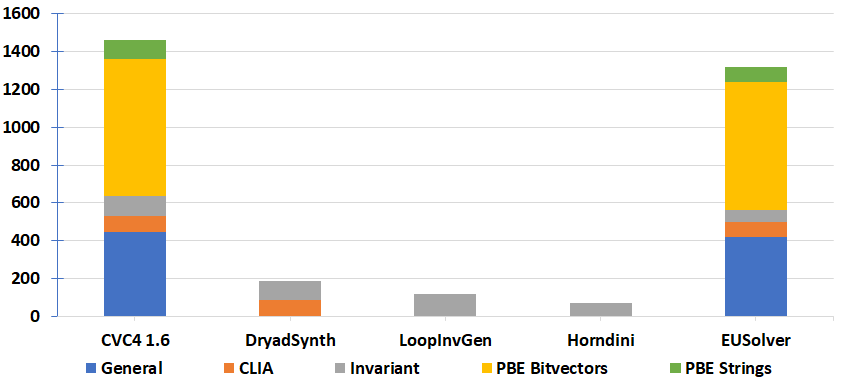
\includegraphics[width=0.95\textwidth]{figures/TotalSolved.png}
% 	\caption{The overall combined results for each solver on benchmarks from all five tracks.}
% 	\label{fig:combinedresults}
% \end{figure}

The primary criterion for winning a track was the number of benchmarks solved,
but we also analyzed the time to solve and the the size of the generated expressions.
The overall score for each solver was computed as $5N + 3F + S$.
Here $N$ denotes the number of benchmarks solved by the solver,
$F$ denotes the number of benchmarks solved among the fastest,
and $S$ denotes the number of benchmarks for which the size of the generated solution was among the shortest.
We used a pseudo-logarithmic scale for $F$ and $S$.
For time to solve, the scale is: $[0,1)$, $[1,3)$, $[3,10)$, $[10,30)$, $[30, 100)$,
$[100,300)$, $[300, 1000)$, $[1000,3600)$, $\geqslant 3600$.
That is, the first ``bucket'' refers to termination in less than one second,
the second to termination in one to three seconds and so on.
We say that a solver solved a certain benchmark \emph{among the fastest}
if the time it took to solve that benchmark is in the same bucket
as that of the solver which solved that benchmark in minimum time.
Similarly, for expression sizes, the pseudo-logarithmic scale we use is:
$[1,10)$, $[10,30)$, $[30,100)$, $[100,300)$, $[300,1000)$, $\geqslant 1000$,
where expression size is the number of nodes in the SyGuS parse-tree.
We also report on the number of benchmarks \emph{solved uniquely} by a solver,
\emph{i.e.} the number of benchmarks which no solver other than the particular solver could solve.

In \Cref{fig:resultsPerTrack}, we show the number of benchmarks solved,
the number of benchmarks solved among the fastest,
and the number of synthesized expressions among the smallest size;
per solver per track.

\begin{figure}
	\begin{center}
		\vspace{3em}
		\begin{minipage}{\textwidth}
			\centering%
			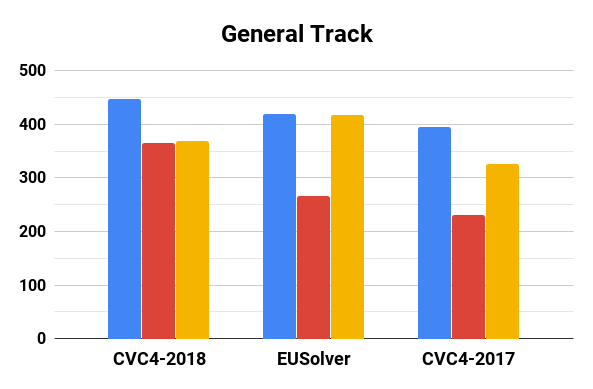
\includegraphics[width=0.5\textwidth]{figures/TrackGeneral.png}%
			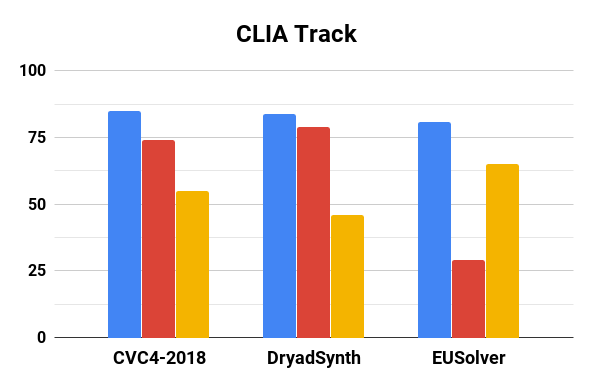
\includegraphics[width=0.5\textwidth]{figures/TrackCLIA.png}
		\end{minipage}
		\\[1cm]
		\begin{minipage}{\textwidth}
			\centering%
			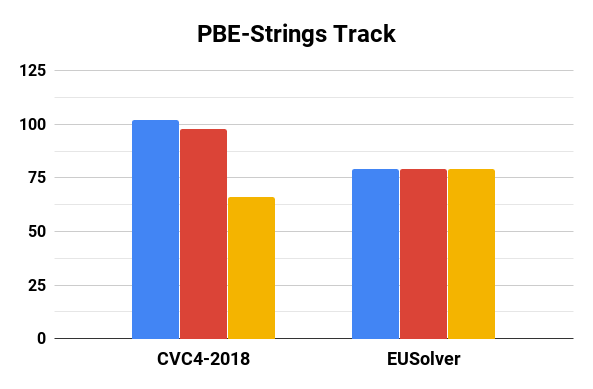
\includegraphics[width=0.5\textwidth]{figures/TrackPBE-Strings.png}%
			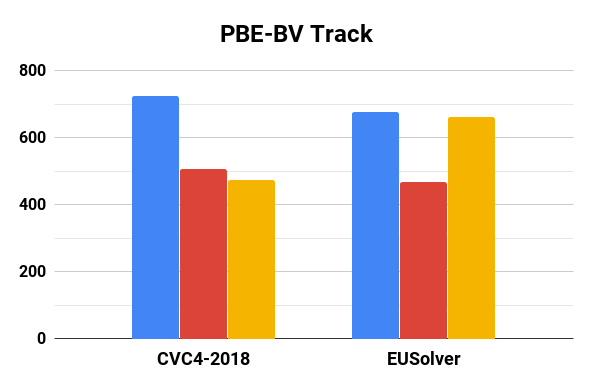
\includegraphics[width=0.5\textwidth]{figures/TrackPBE-BV.png}
		\end{minipage}
		\\[1cm]
		\begin{minipage}{\textwidth}
			\centering%
			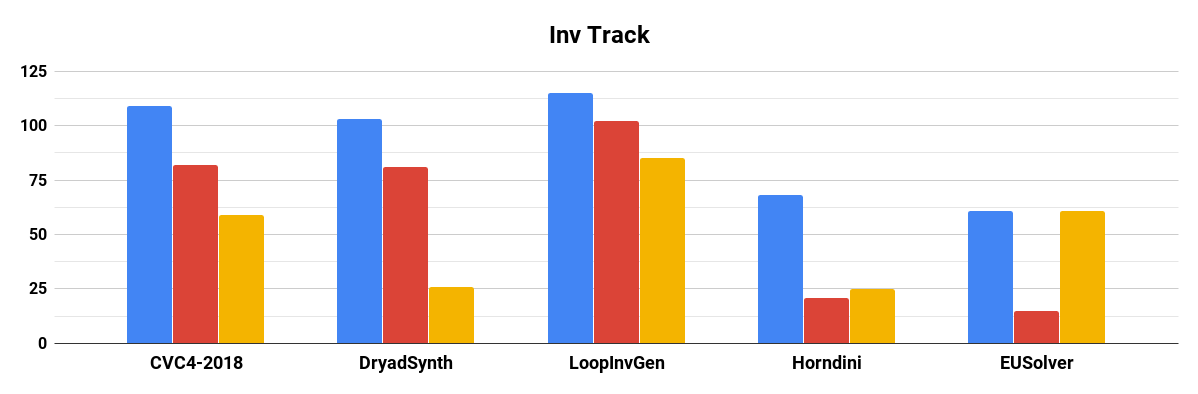
\includegraphics[width=\textwidth]{figures/TrackInv.png}\\[0.5em]
			
\includegraphics[width=0.75\textwidth]{figures/Legend.png}
		\end{minipage}
	\end{center}
	\caption{The number of benchmarks solved by different solvers across all tracks,
			 the number of benchmarks a solver solved among the fastest,
			 and the number of benchmarks for which a solver generated an expression among the smallest size.}
	\label{fig:resultsPerTrack}	
\end{figure}

\paragraph{General Track}
In the general track, \cvcnew\ solved the most number of benchmarks ($448$),
and \eusolvernew\ came second, solving $420$.
We note that the new version \cvcnew\ is significantly better than the previous version \cvclast,
which could only solve $398$ benchmarks.
The same order appears in the number of benchmarks solved among the fastest:
\cvcnew\ with $366$, \eusolvernew\ with $266$, and \cvclast\ with $252$.
Finally, we note that \cvcnew\ is able to solve $12$ benchmarks that no other solver could solve,
and similarly there are $9$ benchmarks that only \eusolver\ could solve.

\begin{table}[t]
	\begin{center}
		\scalebox{0.85}{
		\def\arraystretch{1.125}
		\begin{tabular}{lr||rrrrrrrrrrrr|r}
                                          &	 & \rot{Compiler Optimizations and Bit Vectors}
                                             & \rot{Let and Motion Planning}
                                             & \rot{Invariant Generation with Bounded Ints}
                                             & \rot{Invariant Generation with Unbounded Ints}
                                             & \rot{Multiple Functions}
                                             & \rot{Arrays}
                                             & \rot{Hackers Delight}
                                             & \rot{Integers}
                                             & \rot{Program Repair}
                                             & \rot{ICFP}
                                             & \rot{Cryptographic Circuits}
                                             & \rot{Instruction Selection}
                                             & \textbf{Total} \\\hline \hline
  \multicolumn{2}{r||}{Number of benchmarks} &  32  &   30  &   28  &   28  &   32  &   35  &   69  &   34  &   18  &   50  &   214 &   28  & 598 \\ \hline			 
  \multirow{3}{*}{\textbf{Solved}} & \cvcnew &	16	&   17	&   24	&   24  &	13	&   31	&   62  &	34  &	17  &	50  & 	160 & 	0   & 448 \\
		 			          & \eusolvernew &	16	&   10	&   24	&   23	&   18	&   31  &	53  & 	33  &	14  &	50  &	148 &	0   & 420 \\
 					              & \cvclast &  15	&   15  &   24  &	24  &	12	&   31	&   62	&   34	&   17	&   48	&   116 &	0   & 398 \\ \hline
 \multirow{3}{*}{\textbf{Fastest}} & \cvcnew &	15	&   15	&   22	&   24	&   9	&   31	&   59	&   33  &	16  &	23	&   119 &	0   & 366 \\
 								 & \eusolver &	13  &	1   &	12	&   11	&   14	&   5   &	29	&   15	&   12  & 	45	&   109	&   0   & 266 \\
								  & \cvclast &  12  &	9	&   16	&   14  &	9   &	24	&   60  &	33  &	6	&   20	&   49  & 	0   & 252 \\ \hline
\multirow{3}{*}{\textbf{Uniquely}} & \cvcnew &	1	&   2   & 	0	&   0   & 	0	&   0   & 	0	&   0   &	2	&   0	&   7   &	0   & 12 \\
								 & \eusolver &	3	&   0   &	0   &	0   &	6   &	0	&   0   &	0   &	0   &	0	&   0   &	0   & 9 \\
								  & \cvclast &  0	&   0	&   0   & 	0	&   0   & 	0	&   0   & 	0	&   0   & 	0   &	0	&   0   & 0 \\ \hline			
		\end{tabular}}
	\end{center}
	\captionsetup{skip=0em}
	\caption{The performance of various solvers across all categories of the general track}
	\label{tbl:general-categories}
\end{table}

We partitioned the benchmarks of the general track to a number of categories,
each containing a set of related benchmarks.
The results per category are given in the Table~\ref{tbl:general-categories}.
We observe that \eusolvernew\ preformed significantly better in the ``Multiple Functions'' and ``ICFP'' categories.
While the \cvcnew\ solver preformed better in the other categories,
none of the solvers could solve any of the benchmarks from the ``Instruction Selection'' category.

% \begin{figure}
% 	\begin{center}
% 		\begin{minipage}{1\textwidth}
% 			\centering
% 			\includegraphics[scale=0.9,width=1\textwidth]{Figures/GeneralSolved.png}
% 		\end{minipage}
% 		\\
% 		\vspace{2mm}
% 		\begin{minipage}{1\textwidth}
% 			\centering
% 			\includegraphics[scale=0.9,width=1\textwidth]{Figures/GeneralWon.png}
% 		\end{minipage}
% 	\end{center}
% 	\caption{Percentage of benchmarks solved by the different solvers across all categories of the general track, and the percentage of benchmarks a solver solved among the fastest for that benchmark (according to the logarithmic scale).  }	
% \end{figure}	


\paragraph{Conditional Linear Arithmetic Track}
In the CLIA track, \cvcnew\ and \dryd\ had a close competition.
\cvcnew\ solved $85$ out of $88$ benchmarks, \dryd\ solved $84$ benchmarks, and \eusolvernew\ solved $81$ benchmarks.
In terms of the time to solve, \dryd\ solved $79$ benchmarks among the fastest, \cvcnew\ solved $74$,
followed by \eusolvernew\ which solved $29$ among the fastest.
There were two benchmarks that were solved uniquely by \dryd,
and one that was solved uniquely by \cvcnew.

\paragraph{Invariant Generation Track}
In the invariant generation track, the \lig\ solver solved $115$ out of $127$ benchmarks, \cvcnew\ solved $109$,
\dryd\ solved $103$, \horndini\ solved $68$ and \eusolvernew\ solved $61$ benchmarks.
In terms of the time to solve, \lig\ solved $102$ benchmarks among the fastest, followed by \cvcnew\ which solved $82$,
\dryd\ which solved $81$, \horndini\ which solved $21$, and \eusolvernew\ which solved $15$.
There was one benchmark that was solved by a unique solver -- the \texttt{fib_17n.sl} benchmark solved by \lig. 
\vspace{-0.5em}
\paragraph{Programming By Example (Bit Vectors) Track}
In the PBE track on the theory of bit vectors, the \cvcnew\ solver solved $724$ out of $750$ benchmarks
and \eusolvernew\ solved $677$ benchmarks.
In terms of the time to solve, \cvcnew\ solved $508$ benchmarks among the fastest,
and \eusolvernew\ solved $468$.
However, \eusolvernew\ generates shorter expressions than \cvcnew\ in significantly many cases.
There were four benchmarks that were solved uniquely by \cvcnew,
and one benchmark that was solved uniquely by \eusolvernew.
\vspace{-0.5em}
\paragraph{Programming By Example (Strings) Track}
In the PBE track on the theory of strings, the \cvcnew\ solver solved $102$ out of $118$ benchmarks,
and \eusolvernew\ solved $79$ benchmarks.
In terms of the time to solve, \cvcnew\ solved $98$ benchmarks among the fastest,
and \eusolvernew\ solved $79$.
We note again that \eusolvernew\ generates shorter expressions than \cvcnew\ in several cases.
There were $21$ benchmarks that were solved uniquely by \cvcnew.